\documentclass{article}
\usepackage[utf8]{inputenc}
\usepackage{enumitem}
\usepackage{graphicx}
\usepackage[left=2cm,right=2cm,top=2cm,bottom=2cm]{geometry} %sistema i margini
\usepackage{caption}
\usepackage{subcaption}
\usepackage[colorlinks=true,linkcolor=black]{hyperref}
\usepackage{amsmath}

%per la bibbliografia
%\usepackage{biblatex} %Imports biblatex package
%\addbibresource{reference.bib} %Import the bibliography file


\usepackage[T1]{fontenc}
\usepackage{lmodern}
\usepackage{etoolbox}

\makeatletter
\patchcmd{\@maketitle}{\LARGE}{\Huge}{\typeout{OK 1}}{\typeout{Failed 1}}
\patchcmd{\@maketitle}{\large \lineskip}{\Large \lineskip}{\typeout{OK 2}}{\typeout{Failed 2}}
\makeatother

\title{Networking Lab.2 – Capacity measurements using ping
\\ Laboratorio di Internet}

\author{Riccardo Castiglia 271228 \\  Sebastiano Guzzone 270855 \\ Vincenzo Pio Elia 271173}

\date{31/03/2022}

\begin{document}

\begin{figure}
\centering

\includegraphics[scale=0.125]{polito_logo_2021_blu.jpg}


\end{figure}
\maketitle
\thispagestyle{empty}

\newpage
\tableofcontents %indice
\setcounter{page}{1}
%------------------------------inizio--relazione---------------------------------%

\newpage

\section{Configurazione}
Per la realizzazione di queste esperienza si è fatto uso di un pc con boot da pen-drive con distribuzione Linux fornitaci nel materiale del corso e di un laptop dove è installata una distro linux Xubuntu 20.04 \footnote{tutti i device utilizzati sono forniti di porta ethernet senza adattatori ulteriori} , per creare la rete per quanto riguarda il layer fisico è stato adoperato uno switch di rete, per le prove dove necessario, e cavi Ethernet della lunghezza di 2 metri cadauno per la connessione.
I due host H1, H2 hanno rispettivamente IP 172.16.1.1 e 172.16.1.2 i quali sono stati assegnati da riga di comando tramite comando 
\begin{center}
    \textsf{ sudo ifconfig eno1 172.16.1.h/26}
\end{center}


\section{Aspetti teorici}
Per misurare la velocità di una connessione usando il Round Trip Time ottenuto dal ping è essenziale capire prima il modello sul quale si sta operando, in generale si vuole trovare una grandezza in Mb/s quindi sarà necessario avere notizia riguardo la quantità di dati trasferiti in Mb o MB e di cosa effettivamente si compone l'RTT.
Gli scenari analizzati risultano dunque differenti.

\subsection{Frammentazione}
L'header ip insieme al payload del pacchetto ip formano il payload della trama a Livello 2 che deve necessariamente essere compreso tra 46 Byte \footnote{Necessario per poter attuare i protocolli di collisione} e 1500 Byte \footnote{Dimensione massima impostata dall' MTU per i frame Ethernet}, se a questi si aggiungono i 38 Byte di header ethernet arriviamo all'espressione di D.
Dunque quando S definita come il quantitativo di dati trasmessi a livello applicazione PING supera i  1472 Byte avviene un evento detto \textit{frammentazione}, dunque viene diviso il pacchetto e viene inviata una mole superiore di dati a livello due con eventuale padding se necessario.\\
Alla luce di quanto detto risulta necessaria la definizione di D(S) a tratti e l'uso della funzione di padding.

\subsection{Connessione diretta}
Nel caso di una connessione diretta il Round Trip Time è esprimibile come 
\begin{center}
    $RTT=2 t_{Tx}(D(S)) + 3 t_{elab} + 2 t_{prop} \approx 2 t_{Tx}$
\end{center}
ed è noto inoltre che il tempo di trasmissione (unilaterale da $H_i$ a $H_j$) è pari a 
\begin{center}
    $t_{Tx}= \frac{D(S)}{C} $ \label{t_Tx}
\end{center}
dove C è la capacità del cavo e D la quantità di dati trasmessi a livello fisico che è a sua volta funzione del numero di Bytes inviati a livello applicazione secondo il seguente modello.
\begin{center}
   $$
   D(s)= \begin{cases} (s/1472)\cdot 1538 & $$s\%1472=0$$ \\  (s/1472)\cdot 1538 + ( s\%1472 + padding(s\%1472) + 58) & $$s\%1472\neq0$$
   \end{cases}
   $$
   Dove con "/" si indica la parte intera  del quoziente mentra con "\%" si indica il resto della divisione.
    
   $$
   padding(x)= \begin{cases} 0 & $$ x \ge 18 $$  \\ $$ 18-x $$ & $$ x \le 18 $$
   \end{cases}
   $$
\end{center}

Combinando dunque le due equazioni si ottiene che la capacità del canale può essere nota come
\begin{center}
    $C= \frac{2D(S)}{RTT} $
\end{center}
Dunque analizzando questa formula si può vedere come per arrivare ad un valore più attendibile possibile della stima della capacità si debba prendere il RTT minimo in modo che il contributo della parte considerata trascurabile venga minimizzato.\\
Si noti come con questa sintassi le formule espresse siano valide anche in caso di frammentazione.

\subsection{Connessione tramite switch di rete}
In questa configurazione i due computer sono stati connessi tra di loro per mezzo di due cavi e uno switch di rete. Lo switch nella trasmissione svolge una funzione di store \& forward in quanto deve prima ricevere tutti i byte di un pacchetto prima di poterlo inoltrare nella rete.\\
Nel caso non ci sia frammentazione il Round Trip Time evolve nel modo seguente, mentre restano invariate le definizioni per il $t_{Tx}$ e $D(s)$ fatte nella Sezione \ref{t_Tx}:
\begin{center}
    $RTT=4 t_{Tx}(D(s)) + 3 t_{elab} + 2 t_{prop} \approx 4 t_{Tx}$
\end{center}
dunque la capacita diventa
\begin{center}
    $C= \frac{4D}{RTT}$ 
\end{center} 

Se vi è frammentazione l'RTT cambia in quanto si ha almeno un pacchetto che sicuramente avrà il payload di dimensione pari alla MTU
\begin{center}
    $RTT=2(t_{Tx}(D(s)) + t_{tx}(MTU) ) + \eta \approx 2t_{Tx}(D(s)) + 2t_{tx}(MTU) $
\end{center}
dove $\eta$ è la somma di una serie di contributi di tempo dovuti all'elaborazione dei dati e viene considerata in prima approssimazione trascurabile.
Di conseguenza la capacità C diventa
\begin{center}
    $C=\frac{2D(S)}{RTT-2t_{Tx}(MTU)}$
\end{center}

%----------- Da verificare fino a qua ---------------- %

\section{Ping con connessione diretta, velocità 10 Mb/s} 
In questo caso i due computer sono stati connessi tra di loro esclusivamente tramite un cavo Ethernet.
Dopo aver settato i parametri di trasmissione con la riga:
\begin{center}
    \textsf{ethtool -s [nomeinterfaccia] speed 10 duplex full autoneg on }
\end{center}
è stato lanciato lo script riportato alla Sezione \ref{script_bash}.
I dati raccolti sono stati elaborati tramite \textit{Gnuplot} per arrivare in prima istanza ad un grafico che riporta il Round Trip Time in funzione della dimensione D del pacchetto dopo l'incapsulamento avvento al livello 2.
\begin{center}
    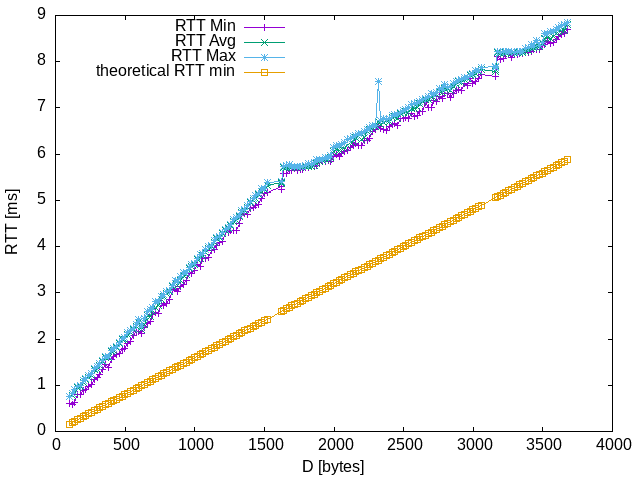
\includegraphics[scale=0.5]{RTT-10Mbps_Direct}
    \label{RTT_D_10_dir}
\end{center}


Dal grafico si può vedere come l'RTT cresca linearmente fino al raggiungimento della MTU (Max Transfer Unit) dove si verifica la frammentazione e l'aggiunta di \textit{padding} al fine di raggiungere la dimensione minima richiesta per il payload. Questi eventi condizionano un "salto" e il successivo tratto costante, per poi riprendere l'andamento lineare fino al raggiungimento del prossimo multiplo della MTU dove si verificherà lo stesso fenomeno.

Plottando i valori ottenuti si può vedere come la velocità tenda a saturare alla capacità attesa all'aumentare di D

\begin{figure}[h!]
\centering
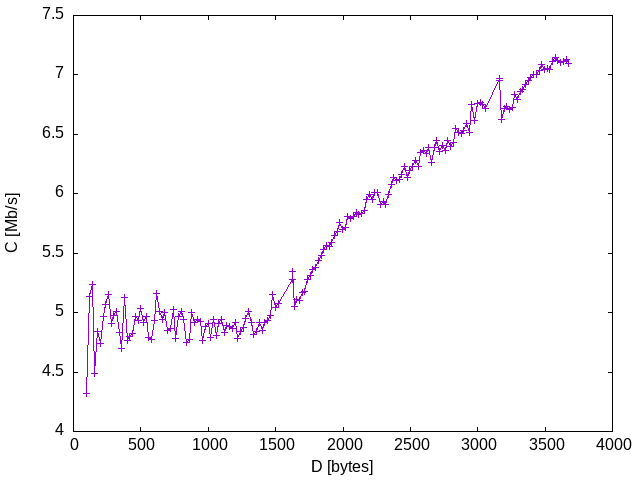
\includegraphics[scale=0.5]{speed-10Mbps_Direct.png}
\caption{C(D), velocità 10 Mb/s}
\label{C_D_10_dir}
\end{figure} 


Dalle misure effettuate come nel caso precedente si può arrivare al plot RTT in funzione di D 


\appendix
\newpage
\section{Script}
\subsection{Bash}
\label{script_bash}
\begin{verbatim}
#!/bin/bash

if test -f "temp_result_ping.txt"; then
    rm "temp_result_ping.txt"   
fi

sequ=”$(seq 16 100 1450) $(seq 1470 1 1500) $(seq 1600 100 10000)”

for i in $sequ; do
    tmp=$(ping -c 10 -s $i -i 0.2 172.16.1.2 | grep "rtt" | cut -d ' ' -f 4 | cut -d '/' -f
    1,2,3 --output-delimiter ' ')
    echo $i $tmp >> temp_result_ping.txt
done
\end{verbatim}
\subsection{Gnuplot}
la fava

\end{document}
